\documentclass[12pt, a4paper]{article}

% Packages
\usepackage[utf8]{inputenc}
\usepackage[T1]{fontenc}
\usepackage{lmodern}
\usepackage[left=2.5cm, right=2.5cm, top=3cm, bottom=3cm]{geometry}
\usepackage{graphicx}
\usepackage{booktabs}
\usepackage{array}
\usepackage{tabularx}
\usepackage{amsmath}
\usepackage{hyperref}
\usepackage{enumitem}
\usepackage{float}
\usepackage{caption}
\usepackage{setspace}
\usepackage{parskip}
\usepackage{fancyhdr}
\usepackage{titlesec}
\usepackage{xcolor}
\usepackage{url}
\usepackage{tikz}
\usepackage{multirow}
\usepackage{colortbl}
\usetikzlibrary{shapes.geometric, arrows.meta, positioning, calc}

% Colours
\definecolor{solarblue}{RGB}{31, 78, 121}
\definecolor{solaramber}{RGB}{180, 100, 20}
\definecolor{solargray}{RGB}{80, 80, 80}
\definecolor{lightgray}{RGB}{245, 245, 245}

% Section formatting
\titleformat{\section}{\large\bfseries\color{solarblue}}{}{0em}{\thesection\quad}[\titlerule]
\titleformat{\subsection}{\normalsize\bfseries\color{solaramber}}{}{0em}{\thesubsection\quad}
\titleformat{\subsubsection}{\normalsize\itshape\color{solargray}}{}{0em}{\thesubsubsection\quad}

% Hyperref config
\hypersetup{
    colorlinks=true,
    linkcolor=solarblue,
    urlcolor=solaramber,
    citecolor=solarblue
}

% Header/Footer
\pagestyle{fancy}
\fancyhf{}
\fancyhead[L]{\small\textit{SolarIntel}}
\fancyhead[R]{\small\textit{Solar Energy Generation Prediction}}
\fancyfoot[C]{\thepage}
\renewcommand{\headrulewidth}{0.4pt}

% Spacing
\onehalfspacing
\setlength{\parindent}{0pt}

% Title Page
\begin{document}

\begin{titlepage}
    \centering
    \vspace*{1.5cm}

    {\huge\bfseries\color{solarblue} SolarIntel}\\[0.6cm]
    {\Large\color{solaramber} Solar Energy Generation Prediction}\\[0.3cm]
    {\large Using EMHIRES and NASA POWER Data}\\[0.4cm]
    \rule{\linewidth}{1.5pt}\\[0.8cm]

    {\large\textbf{Project Report}}

    \vspace{1.5cm}

    \begin{tabular}{rl}
        \textbf{Live Demo:} & \url{https://huggingface.co/spaces/priyanshutomar2024/SolarIntel} \\[4pt]
        \textbf{Domain:} & Machine Learning, Renewable Energy, Agentic AI \\[4pt]
        \textbf{Models:} & Linear Regression, Random Forest Regressor \\[4pt]
        \textbf{Deployment:} & Streamlit on Hugging Face Spaces \\[4pt]
        \textbf{Coverage:} & 29 European Countries, 2001--2015, Hourly \\
    \end{tabular}

    \vspace{2cm}

    \vfill
    {\large \today}
\end{titlepage}

% Front matter — roman numerals
\pagenumbering{roman}

% Table of Contents
\newpage
{\singlespacing
\tableofcontents
}
\newpage

% Abstract
\begin{abstract}
\noindent
Accurate forecasting of solar energy generation is essential for grid balancing, energy market operations, and renewable infrastructure planning across Europe. This report presents \textbf{SolarIntel}, an end-to-end machine learning system that predicts hourly solar capacity factors for 29 European countries by fusing 15 years of photovoltaic generation data from the European Commission's EMHIRES dataset with satellite-derived meteorological observations from NASA's POWER API. The resulting dataset comprises approximately 3.8 million hourly records and 34 features. Two regression models are trained and evaluated: a Linear Regression baseline ($R^2 = 0.788$) and a Random Forest Regressor ($R^2 = 0.911$). The superior model is deployed through an interactive Streamlit web application hosted on Hugging Face Spaces, enabling real-time prediction, 24-hour generation profiling, and cross-country comparison. Building on this ML foundation, Phase~2 introduces an Agentic AI Grid Advisor: a LangGraph-based multi-agent pipeline that fetches live weather forecasts, performs deterministic risk analysis, retrieves expert knowledge via Retrieval-Augmented Generation (RAG), and generates structured LLM recommendations tailored to grid operators and transmission system planners.
\end{abstract}

% Main matter — arabic numerals, restart from 1
\clearpage
\pagenumbering{arabic}

% Section 1
\section{Introduction}

Solar energy is one of the fastest-growing renewable energy sources globally. Accurate forecasting of solar energy generation is critical for grid stability, energy trading, and infrastructure planning. The variability of solar output, driven by weather conditions, geographic location, and time of day, makes prediction a non-trivial challenge.

This project, \textbf{SolarIntel}, addresses this challenge by building an end-to-end machine learning pipeline that predicts hourly solar energy capacity factors across 29 European countries. The system fuses 15 years of solar generation data from the European Commission's EMHIRES dataset with hourly meteorological observations from NASA's POWER API. Two regression models are trained, evaluated, and compared. The best-performing model is deployed through an interactive Streamlit web application hosted on Hugging Face Spaces.

\subsection{Objectives}

\begin{itemize}[noitemsep]
    \item Collect, clean, and merge solar generation and weather datasets spanning 2001--2015.
    \item Engineer temporal and geographic features suitable for regression modelling.
    \item Train and evaluate two regression models: Linear Regression and Random Forest Regressor.
    \item Deploy the trained model as an interactive web application for real-time predictions.
    \item Extend the system with an agentic AI pipeline that provides automated grid risk analysis and operator-facing recommendations using live weather forecasts.
\end{itemize}

\subsection{Scope}

The pipeline covers 29 European countries at hourly resolution. The target variable is Capacity Factor, a normalised measure of solar output ranging from 0.0 (no generation) to 1.0 (maximum rated output). The final dataset contains approximately 3.8 million rows and 34 features. Phase~2 extends the system with a four-node LangGraph agent pipeline and RAG-enhanced recommendation engine.

% Section 2
\newpage
\section{Data Sources}

Two primary datasets are used. Both are publicly available.

\subsection{EMHIRES PV Dataset}

The European Meteorological-derived High-resolution RES generation time series for present and future scenarios (EMHIRES) dataset is published by the European Commission's Joint Research Centre (JRC). The PV module provides hourly solar capacity factors for European countries from 1986 to 2015.

\begin{table}[H]
    \centering
    \caption{EMHIRES PV Dataset Summary}
    \begin{tabular}{ll}
        \toprule
        \textbf{Attribute} & \textbf{Detail} \\
        \midrule
        Source & European Commission, JRC \\
        Temporal Coverage & 1986--2015 (hourly) \\
        Spatial Coverage & 29 European countries \\
        Format & Wide-format CSV (countries as columns) \\
        Target Variable & Capacity Factor (0.0--1.0) \\
        \bottomrule
    \end{tabular}
\end{table}

The dataset is in wide format with each column representing a country code (e.g., AT for Austria, ES for Spain). Each row corresponds to one hour. The data was filtered to the 2001--2015 range to align with the availability of NASA weather data.

\subsection{NASA POWER API}

The Prediction Of Worldwide Energy Resources (POWER) project by NASA provides satellite-derived meteorological data. Hourly observations were fetched via the POWER API for all 29 EMHIRES countries using geographic centroids.

\begin{table}[H]
    \centering
    \caption{NASA POWER Weather Parameters}
    \begin{tabular}{lll}
        \toprule
        \textbf{API Parameter} & \textbf{Renamed To} & \textbf{Unit} \\
        \midrule
        ALLSKY\_SFC\_SW\_DWN & Irradiance & W/m\textsuperscript{2} \\
        T2M & Temperature & \textdegree C \\
        WS2M & Wind Speed & m/s \\
        \bottomrule
    \end{tabular}
\end{table}

Data was collected for each country and each year (2001--2015) individually, with a 0.5-second delay between requests to respect API rate limits. The full fetch takes approximately 20 minutes due to the volume of requests (29 countries $\times$ 15 years = 435 API calls).

% Section 3
\newpage
\section{Data Pipeline}

The pipeline follows a sequential flow: data loading, cleaning, transformation, merging, encoding, and export. Each stage is implemented as a standalone Python module and also consolidated in a single end-to-end script. Figure~\ref{fig:pipeline} illustrates the full architecture.

\begin{figure}[H]
\centering
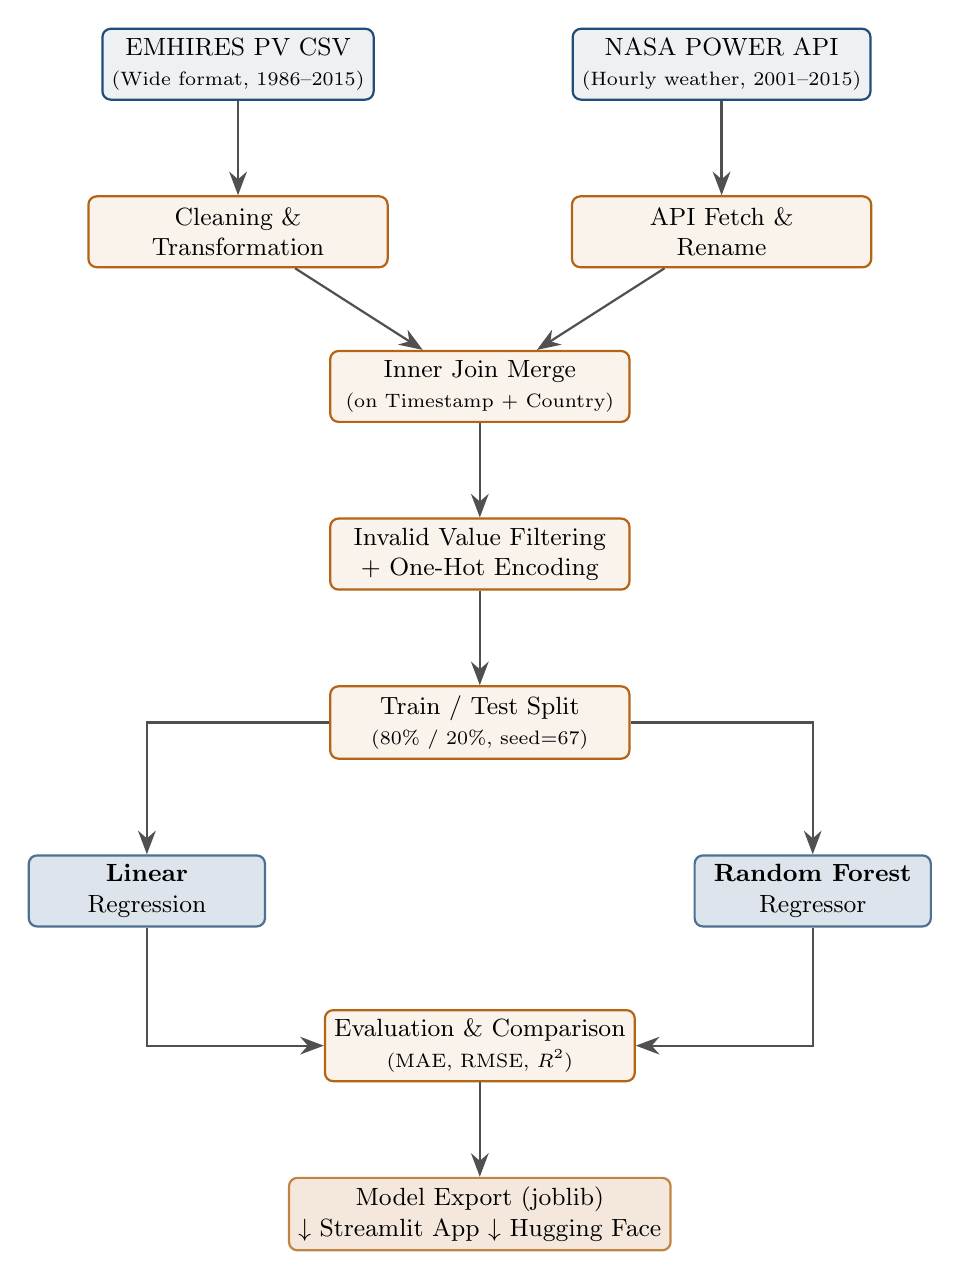
\begin{tikzpicture}[
    node distance=1.2cm and 2.5cm,
    every node/.style={font=\small},
    databox/.style={rectangle, draw=solarblue, fill=solarblue!8, rounded corners=3pt, minimum width=3.2cm, minimum height=0.9cm, align=center, thick},
    procbox/.style={rectangle, draw=solaramber, fill=solaramber!8, rounded corners=3pt, minimum width=3.8cm, minimum height=0.9cm, align=center, thick},
    modelbox/.style={rectangle, draw=solarblue!80, fill=solarblue!15, rounded corners=3pt, minimum width=3cm, minimum height=0.9cm, align=center, thick},
    deploybox/.style={rectangle, draw=solaramber!80, fill=solaramber!15, rounded corners=3pt, minimum width=4cm, minimum height=0.9cm, align=center, thick},
    arrow/.style={-{Stealth[length=3mm]}, thick, color=solargray}
]

% Data sources
\node[databox] (emhires) {EMHIRES PV CSV\\{\scriptsize (Wide format, 1986--2015)}};
\node[databox, right=of emhires] (nasa) {NASA POWER API\\{\scriptsize (Hourly weather, 2001--2015)}};

% Processing
\node[procbox, below=of emhires] (clean) {Cleaning \&\\Transformation};
\node[procbox, below=of nasa] (fetch) {API Fetch \&\\Rename};

% Merge
\node[procbox, below=1.5cm of $(clean)!0.5!(fetch)$] (merge) {Inner Join Merge\\{\scriptsize (on Timestamp + Country)}};

% Filter + Encode
\node[procbox, below=of merge] (filter) {Invalid Value Filtering\\+ One-Hot Encoding};

% Split
\node[procbox, below=of filter] (split) {Train / Test Split\\{\scriptsize (80\% / 20\%, seed=67)}};

% Models
\node[modelbox, below left=1.2cm and 0.8cm of split] (lr) {\textbf{Linear}\\Regression};
\node[modelbox, below right=1.2cm and 0.8cm of split] (rfr) {\textbf{Random Forest}\\Regressor};

% Evaluation
\node[procbox, below=1.5cm of $(lr)!0.5!(rfr)$] (eval) {Evaluation \& Comparison\\{\scriptsize (MAE, RMSE, $R^2$)}};

% Export + Deploy
\node[deploybox, below=of eval] (deploy) {Model Export (joblib)\\$\downarrow$ Streamlit App $\downarrow$ Hugging Face};

% Arrows
\draw[arrow] (emhires) -- (clean);
\draw[arrow] (nasa) -- (fetch);
\draw[arrow] (clean) -- (merge);
\draw[arrow] (fetch) -- (merge);
\draw[arrow] (merge) -- (filter);
\draw[arrow] (filter) -- (split);
\draw[arrow] (split) -| (lr);
\draw[arrow] (split) -| (rfr);
\draw[arrow] (lr) |- (eval);
\draw[arrow] (rfr) |- (eval);
\draw[arrow] (eval) -- (deploy);

\end{tikzpicture}
\caption{SolarIntel Pipeline Architecture}
\label{fig:pipeline}
\end{figure}

\subsection{Cleaning and Transformation}

The raw EMHIRES CSV is in wide format with no explicit timestamps. Timestamps were generated programmatically starting from 1 January 1986 at hourly frequency. The data was then reshaped from wide to long format using \texttt{pd.melt()}, producing three columns: \texttt{Timestamp}, \texttt{Country}, and \texttt{Capacity\_Factor}.

Key operations:
\begin{itemize}[noitemsep]
    \item Timestamp generation using \texttt{pd.date\_range()} from 1986-01-01, hourly frequency.
    \item Wide-to-long reshaping via \texttt{pd.melt()}.
    \item Filtering to 2001--2015 to match NASA POWER data availability.
    \item Extraction of temporal features: \texttt{Hour} (0--23) and \texttt{Month} (1--12).
\end{itemize}

\subsection{Merging}

The EMHIRES long-format data and NASA weather data were merged on \texttt{Timestamp} and \texttt{Country} using an inner join. This ensures every row has both a capacity factor value and corresponding weather observations. Float64 weather columns were downcast to float32 to reduce memory consumption.

Post-merge filtering removed invalid weather readings:
\begin{itemize}[noitemsep]
    \item Irradiance $< 0$ (physically impossible).
    \item Temperature $= -999.0$ (NASA fill value for missing data).
    \item Wind Speed $= -999.0$ (NASA fill value for missing data).
\end{itemize}

\subsection{Encoding}

The categorical \texttt{Country} column was one-hot encoded using \texttt{pd.get\_dummies()}, producing 29 binary indicator columns (e.g., \texttt{Country\_AT}, \texttt{Country\_ES}). This is necessary because the regression models require numerical input. The resulting dataset was exported as \texttt{merged\_encoded.csv}.

\subsection{Final Dataset Summary}

\begin{table}[H]
    \centering
    \caption{Final Dataset Characteristics}
    \begin{tabular}{ll}
        \toprule
        \textbf{Property} & \textbf{Value} \\
        \midrule
        Total Rows & $\sim$3,812,690 \\
        Total Features & 34 \\
        Numerical Features & 5 (Hour, Month, Irradiance, Temperature, Wind Speed) \\
        Encoded Features & 29 (one per country) \\
        Target Variable & Capacity Factor \\
        Time Range & 2001--2015 (hourly) \\
        Countries & 29 European nations \\
        \bottomrule
    \end{tabular}
\end{table}

% Section 4
\newpage
\section{Feature Engineering}

Feature engineering was kept deliberate, deriving only features with clear physical relevance to solar generation.

\begin{table}[H]
    \centering
    \caption{Feature Descriptions}
    \begin{tabularx}{\textwidth}{lllX}
        \toprule
        \textbf{Feature} & \textbf{Type} & \textbf{Range} & \textbf{Rationale} \\
        \midrule
        Hour & Temporal & 0--23 & Solar output follows a diurnal cycle peaking around midday. \\
        Month & Temporal & 1--12 & Captures seasonal variation in daylight hours and sun angle. \\
        Irradiance & Weather & $\geq$ 0 W/m\textsuperscript{2} & Primary driver of photovoltaic output. \\
        Temperature & Weather & \textdegree C & Higher temperatures reduce PV panel efficiency. \\
        Wind Speed & Weather & $\geq$ 0 m/s & Affects panel cooling and efficiency indirectly. \\
        Country\_* & Categorical & 0 or 1 & Geographic identity capturing latitude, climate, and installed capacity differences. \\
        \bottomrule
    \end{tabularx}
\end{table}

The feature set was intentionally kept minimal to avoid overfitting and to maintain interpretability. Irradiance is the strongest predictor, with Hour and Month providing temporal context. The country one-hot encoding allows the model to learn location-specific baselines.

% Section 5
\newpage
\section{Model Training and Configuration}

Two regression models were trained and compared. Both are provided by scikit-learn.

\subsection{Train-Test Split}

The dataset was split into 80\% training and 20\% testing subsets using \texttt{train\_test\_split()} with \texttt{random\_state=67} for reproducibility. The \texttt{Timestamp} and \texttt{Capacity\_Factor} columns were excluded from the feature matrix.

\begin{table}[H]
    \centering
    \caption{Data Split}
    \begin{tabular}{ll}
        \toprule
        \textbf{Set} & \textbf{Samples} \\
        \midrule
        Training & 3,050,152 \\
        Testing & 762,538 \\
        Total & 3,812,690 \\
        \bottomrule
    \end{tabular}
\end{table}

\subsection{Linear Regression}

A standard Ordinary Least Squares (OLS) regression model. It assumes a linear relationship between the features and the target variable. This model serves as a baseline due to its simplicity and interpretability.

\clearpage
\subsection{Random Forest Regressor}

An ensemble method that fits multiple decision trees on bootstrapped subsets of the data and averages their predictions. It captures non-linear relationships and feature interactions that linear regression cannot.

\begin{table}[H]
    \centering
    \caption{Random Forest Hyperparameters}
    \begin{tabular}{ll}
        \toprule
        \textbf{Parameter} & \textbf{Value} \\
        \midrule
        n\_estimators & 100 \\
        max\_depth & 12 \\
        random\_state & 67 \\
        n\_jobs & -1 (all CPU cores) \\
        \bottomrule
    \end{tabular}
\end{table}

Both trained models were serialised using \texttt{joblib} and exported as \texttt{.pkl} files for deployment.

% Section 6
\newpage
\section{Model Evaluation}

Three standard regression metrics were used to evaluate both models on the held-out test set.

\subsection{Evaluation Metrics}

\textbf{Mean Absolute Error (MAE):} The average absolute difference between predicted and actual values. Lower is better.
\begin{equation}
    \text{MAE} = \frac{1}{n} \sum_{i=1}^{n} |y_i - \hat{y}_i|
\end{equation}

\textbf{Root Mean Squared Error (RMSE):} The square root of the average squared differences. Penalises larger errors more heavily than MAE.
\begin{equation}
    \text{RMSE} = \sqrt{\frac{1}{n} \sum_{i=1}^{n} (y_i - \hat{y}_i)^2}
\end{equation}

\textbf{R-Squared ($R^2$):} The proportion of variance in the target explained by the model. A value of 1.0 indicates perfect prediction.
\begin{equation}
    R^2 = 1 - \frac{\sum_{i=1}^{n} (y_i - \hat{y}_i)^2}{\sum_{i=1}^{n} (y_i - \bar{y})^2}
\end{equation}

\subsection{Results}

\begin{table}[H]
    \centering
    \caption{Test Set Performance Comparison}
    \begin{tabular}{lccc}
        \toprule
        \textbf{Model} & \textbf{MAE} & \textbf{RMSE} & \textbf{$R^2$} \\
        \midrule
        Linear Regression & 0.0534 & 0.0845 & 0.7880 \\
        \rowcolor{solarblue!8} Random Forest Regressor & \textbf{0.0280} & \textbf{0.0547} & \textbf{0.9112} \\
        \bottomrule
    \end{tabular}
\end{table}

\begin{table}[H]
    \centering
    \caption{Training Set Performance Comparison}
    \begin{tabular}{lccc}
        \toprule
        \textbf{Model} & \textbf{MAE} & \textbf{RMSE} & \textbf{$R^2$} \\
        \midrule
        Linear Regression & 0.0534 & 0.0844 & 0.7882 \\
        \rowcolor{solarblue!8} Random Forest Regressor & \textbf{0.0278} & \textbf{0.0543} & \textbf{0.9123} \\
        \bottomrule
    \end{tabular}
\end{table}

\subsection{Analysis}

The Random Forest Regressor significantly outperforms Linear Regression across all three metrics. Key observations:

\begin{itemize}[noitemsep]
    \item The Random Forest achieves an $R^2$ of 0.9112 on the test set, explaining over 91\% of the variance in capacity factor. Linear Regression explains approximately 79\%.
    \item The MAE for Random Forest (0.0280) is roughly half that of Linear Regression (0.0534), meaning its average prediction error is about 2.8 percentage points on the capacity factor scale.
    \item The close alignment between training and testing metrics for Linear Regression (MAE: 0.0534 vs 0.0534) confirms it is not overfitting, but its linear assumption limits its ceiling.
    \item The close alignment between training $R^2$ (0.9123) and test $R^2$ (0.9112) confirms that the Random Forest is generalising well and not overfitting, aided by the \texttt{max\_depth=12} constraint.
\end{itemize}

% Section 7
\newpage
\section{Deployment}

The trained models are deployed through a Streamlit web application hosted on Hugging Face Spaces.

\subsection{Application Architecture}

The application consists of two main components:

\begin{itemize}[noitemsep]
    \item \textbf{model\_loader.py} -- Handles model loading from \texttt{.pkl} files using \texttt{joblib}, constructs feature vectors from user inputs, and returns capacity factor predictions.
    \item \textbf{app.py} -- The Streamlit frontend providing interactive controls (country selection, weather parameters, time inputs) and visualisations (prediction gauges, 24-hour generation profiles, country comparisons, and the Grid Advisor panel).
\end{itemize}

\subsection{Features}

The deployed application provides three tabs:

\begin{itemize}[noitemsep]
    \item \textbf{Prediction tab} -- Real-time capacity factor prediction based on user-selected country, time, and weather conditions. Includes 24-hour generation profile simulation and installed capacity scaling to convert capacity factor to absolute power output (kW).
    \item \textbf{Country Comparison tab} -- Benchmarking solar potential across regions with model selection toggle between Linear Regression and Random Forest Regressor.
    \item \textbf{Grid Advisor tab} -- Agentic AI pipeline (Phase~2) that fetches live weather, runs ML predictions, performs risk analysis, retrieves expert knowledge via RAG, and generates structured LLM recommendations. Described fully in Sections~\ref{sec:gridadvisor}--\ref{sec:qualitative}.
\end{itemize}

\subsection{Hosting}

The application is publicly accessible at:

\begin{center}
    \url{https://huggingface.co/spaces/priyanshutomar2024/SolarIntel}
\end{center}

Hugging Face Spaces provides free hosting for Streamlit applications with persistent storage for model files.

% -----------------------------------------------------------------------
% PHASE 2 SECTIONS
% -----------------------------------------------------------------------

% Section 7a
\newpage
\section{Agentic AI System --- Grid Advisor}
\label{sec:gridadvisor}

\subsection{Motivation}

The Phase~1 ML pipeline answers one question: \textit{given weather inputs and a country, what will the capacity factor be?} This is sufficient for energy market participants who need point estimates, but it is insufficient for grid operators and transmission system operators (TSOs) who must act on that information. Grid operators require answers to questions such as: Will generation ramp down sharply this afternoon? When should reserves be pre-positioned? Which balancing mechanism is most appropriate for the expected variability?

Rule-based threshold systems can flag obvious events (e.g., generation below 10\,kW), but they cannot synthesise contextual knowledge, adapt their recommendations to market structure, or explain their reasoning in operator-appropriate language. A large language model (LLM), conversely, has broad knowledge of grid operations and balancing mechanisms but cannot access real-time forecast data or the trained Random Forest model.

The Grid Advisor bridges this gap by composing both capabilities inside a directed agentic pipeline: deterministic computation (weather fetch, ML inference, risk arithmetic) feeds structured context into a retrieval-augmented LLM, which produces operator-facing recommendations grounded in real data.

\subsection{Pipeline Overview}

The Grid Advisor is implemented as a four-node \texttt{StateGraph} using LangGraph. Each node receives the full pipeline state, performs a single well-defined operation, and writes its outputs back to state fields before passing control to the next node. The nodes execute sequentially in a directed acyclic graph (DAG); there are no cycles or conditional branches in the current implementation.

\begin{table}[H]
    \centering
    \caption{LangGraph Node Responsibilities}
    \begin{tabularx}{\textwidth}{llX}
        \toprule
        \textbf{Node} & \textbf{Type} & \textbf{Responsibility} \\
        \midrule
        \texttt{forecast\_node} & Deterministic & Fetches 24-hour weather from Open-Meteo; calls trained Random Forest 24 times to build the hourly CF profile. \\
        \texttt{risk\_analysis\_node} & Deterministic & Computes variability score, low-generation hours, and ramp events; emits plain-English risk flags. \\
        \texttt{rag\_retrieval\_node} & Retrieval & Queries ChromaDB vector store with risk-aware query; returns top-4 semantically relevant knowledge-base chunks. \\
        \texttt{recommendation\_node} & LLM & Sends hourly profile, risk flags, and RAG chunks to an OpenRouter LLM; parses JSON response into structured recommendations. \\
        \bottomrule
    \end{tabularx}
\end{table}

\subsection{LangGraph StateGraph Design}

LangGraph models agent pipelines as typed state machines. The shared state object (\texttt{GridAdvisorState}) is a \texttt{TypedDict} that every node reads from and writes to. Nodes declare no explicit inter-node dependencies; the framework executes them in the order they are connected by \texttt{add\_edge()} calls. This design provides three properties valuable in production:

\begin{itemize}[noitemsep]
    \item \textbf{Auditability} -- every intermediate result (weather forecast, risk flags, RAG chunks) is preserved in state and can be logged or inspected without re-running the pipeline.
    \item \textbf{Replaceability} -- any node can be swapped (e.g., replacing Open-Meteo with a paid NWP provider) without touching the other nodes, because the state schema acts as the interface contract.
    \item \textbf{Testability} -- each node is a pure Python function accepting and returning a dict-like object, enabling unit tests without running the full graph.
\end{itemize}

The graph is compiled once at application startup (cached by \texttt{@st.cache\_resource}) and invoked per user request with a fresh initial state populated from the Streamlit sidebar inputs.

\clearpage
\subsection{Pipeline Architecture Diagram}

Figure~\ref{fig:advisor} shows the four-node pipeline and the state fields produced at each stage.

\begin{figure}[H]
\centering
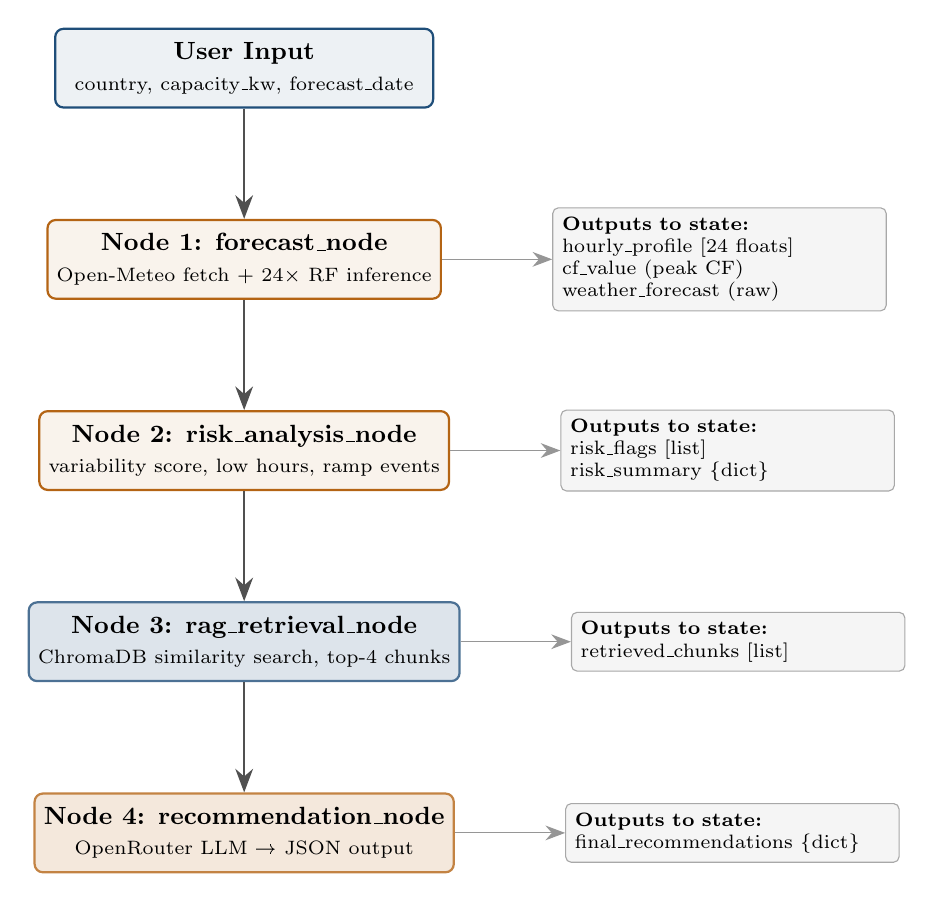
\begin{tikzpicture}[
    node distance=1.4cm,
    every node/.style={font=\small},
    databox/.style={rectangle, draw=solarblue, fill=solarblue!8, rounded corners=3pt,
                    minimum width=4.8cm, minimum height=1.0cm, align=center, thick},
    procbox/.style={rectangle, draw=solaramber, fill=solaramber!8, rounded corners=3pt,
                    minimum width=4.8cm, minimum height=1.0cm, align=center, thick},
    modelbox/.style={rectangle, draw=solarblue!80, fill=solarblue!15, rounded corners=3pt,
                     minimum width=4.8cm, minimum height=1.0cm, align=center, thick},
    deploybox/.style={rectangle, draw=solaramber!80, fill=solaramber!15, rounded corners=3pt,
                      minimum width=4.8cm, minimum height=1.0cm, align=center, thick},
    sidenote/.style={rectangle, draw=solargray!50, fill=lightgray, rounded corners=2pt,
                     minimum width=4.0cm, align=left, font=\scriptsize, text width=4.0cm},
    arrow/.style={-{Stealth[length=3mm]}, thick, color=solargray},
    sidearrow/.style={-{Stealth[length=2.5mm]}, thin, color=solargray!60}
]

% Input
\node[databox] (input) {\textbf{User Input}\\{\scriptsize country, capacity\_kw, forecast\_date}};

% Node 1
\node[procbox, below=of input] (n1) {\textbf{Node 1: forecast\_node}\\{\scriptsize Open-Meteo fetch + 24$\times$ RF inference}};

% Node 2
\node[procbox, below=of n1] (n2) {\textbf{Node 2: risk\_analysis\_node}\\{\scriptsize variability score, low hours, ramp events}};

% Node 3
\node[modelbox, below=of n2] (n3) {\textbf{Node 3: rag\_retrieval\_node}\\{\scriptsize ChromaDB similarity search, top-4 chunks}};

% Node 4
\node[deploybox, below=of n3] (n4) {\textbf{Node 4: recommendation\_node}\\{\scriptsize OpenRouter LLM \textrightarrow{} JSON output}};

% Side notes
\node[sidenote, right=1.4cm of n1] (sn1)
    {\textbf{Outputs to state:}\\hourly\_profile [24 floats]\\cf\_value (peak CF)\\weather\_forecast (raw)};
\node[sidenote, right=1.4cm of n2] (sn2)
    {\textbf{Outputs to state:}\\risk\_flags [list]\\risk\_summary \{dict\}};
\node[sidenote, right=1.4cm of n3] (sn3)
    {\textbf{Outputs to state:}\\retrieved\_chunks [list]};
\node[sidenote, right=1.4cm of n4] (sn4)
    {\textbf{Outputs to state:}\\final\_recommendations \{dict\}};

% Main arrows
\draw[arrow] (input) -- (n1);
\draw[arrow] (n1) -- (n2);
\draw[arrow] (n2) -- (n3);
\draw[arrow] (n3) -- (n4);

% Side arrows
\draw[sidearrow] (n1.east) -- (sn1.west);
\draw[sidearrow] (n2.east) -- (sn2.west);
\draw[sidearrow] (n3.east) -- (sn3.west);
\draw[sidearrow] (n4.east) -- (sn4.west);

\end{tikzpicture}
\caption{Grid Advisor LangGraph pipeline: four sequential nodes with state outputs annotated.}
\label{fig:advisor}
\end{figure}

\clearpage
\subsection{GridAdvisorState Schema}

The complete shared state is defined as a \texttt{TypedDict} in \texttt{Agent\_Pipeline/state.py}. Table~\ref{tab:state} lists all fields and their roles.

\begin{table}[H]
    \centering
    \caption{GridAdvisorState fields}
    \label{tab:state}
    \begin{tabularx}{\textwidth}{llX}
        \toprule
        \textbf{Field} & \textbf{Type} & \textbf{Purpose} \\
        \midrule
        \texttt{country} & str & ISO 3166-1 alpha-2 country code \\
        \texttt{capacity\_kw} & float & Installed solar capacity in kilowatts \\
        \texttt{model\_name} & str & Model selector (Random Forest) \\
        \texttt{forecast\_date} & str & Target forecast date string \\
        \texttt{weather\_forecast} & list & Raw 24-hour Open-Meteo response \\
        \texttt{cf\_value} & float & Peak capacity factor from hourly profile \\
        \texttt{hourly\_profile} & list & 24 capacity factor values, one per hour \\
        \texttt{monthly\_profile} & list & 12 monthly CFs at peak hour conditions \\
        \texttt{risk\_summary} & dict & Variability score, low hours, ramp events \\
        \texttt{risk\_flags} & list & Plain-English risk descriptions \\
        \texttt{retrieved\_chunks} & list & Top-4 RAG chunks with source labels \\
        \texttt{final\_recommendations} & dict & Structured LLM JSON output \\
        \texttt{error} & Optional[str] & Exception detail if any node fails \\
        \bottomrule
    \end{tabularx}
\end{table}

% Section 7b
\newpage
\section{Forecast and Risk Analysis Nodes}
\label{sec:forecastrisk}

\subsection{forecast\_node: Open-Meteo Integration}

The forecast node fetches real hourly weather for the selected country from the Open-Meteo API, a free and open meteorological data service requiring no API key. The request targets three parameters: \texttt{shortwave\_radiation} (W/m\textsuperscript{2}), \texttt{temperature\_2m} (\textdegree C), and \texttt{wind\_speed\_10m} (m/s at 10\,m height, reported in m/s via the \texttt{wind\_speed\_unit=ms} parameter). The full HTTP request construction and response parsing logic is implemented in \texttt{Agent\_Pipeline/weather/fetcher.py}.

The API is called with \texttt{forecast\_days=16} to support the full 1--15 day forecast range exposed in the UI. The target day is extracted by slicing the response at \texttt{day\_offset * 24} (e.g.\ \texttt{day\_offset=1} yields hours 24--47, i.e.\ tomorrow). Country coordinates are taken from a hardcoded centroid dictionary (\texttt{COUNTRY\_COORDS}, 29 entries) that mirrors the spatial reference used during training. After fetching, the node iterates over all 24 hours and calls \texttt{predict\_capacity\_factor()} once per hour. The result is a list of 24 floats written to \texttt{hourly\_profile}, with the maximum value written to \texttt{cf\_value}.

The node also computes a \texttt{monthly\_profile}: 12 capacity factor estimates for months 1--12 at the peak hour's weather conditions. This provides a seasonal reference baseline stored in state for downstream use.

This 24-call loop is deliberately synchronous. Random Forest inference is fast (sub-millisecond per call), so parallelism would add overhead without meaningful latency reduction.

\subsection{risk\_analysis\_node: Deterministic Risk Computation}

The risk node operates entirely in Python with no external calls. It receives the \texttt{hourly\_profile} from state and computes three risk indicators.

\subsubsection{Variability Score}

The variability score is a normalised mean absolute ramp rate:

\begin{equation}
    V = \frac{1}{(H-1) \cdot \text{CF}_{\max}} \sum_{h=1}^{H-1} \left| \text{CF}_h - \text{CF}_{h-1} \right|
\label{eq:variability}
\end{equation}

where $H = 24$ is the number of hours and $\text{CF}_{\max}$ is the peak capacity factor in the profile. The denominator normalises by both the number of transitions and the peak output, making the score scale-invariant: a 160\,kW system and a 1\,MW system experiencing identical relative fluctuations will yield the same $V$.

This is preferable to raw standard deviation for two reasons. First, standard deviation measures dispersion around the mean, which conflates the natural day/night cycle (large expected variance) with intra-day instability (operationally important variance). Second, the normalisation by $\text{CF}_{\max}$ ensures the score is meaningful even on days with low absolute generation, where raw ramp magnitudes are small but relative instability may still be high.

\subsubsection{Low-Generation Hours}

Low-generation hours are defined as hours where:
\begin{equation}
    \text{CF}_h < 0.10 \times \text{CF}_{\max}
\end{equation}

Using a relative threshold (10\% of peak) rather than an absolute value (e.g., $\text{CF} < 0.05$) is essential for correct behaviour across geographies. Southern European countries regularly achieve $\text{CF}_{\max} > 0.7$, while Nordic countries in winter may peak at 0.15. An absolute threshold would flag all Nordic daylight hours as low-generation, obscuring the genuinely useful signal.

\subsubsection{Ramp Events}

A ramp event is detected when the absolute hour-on-hour change in capacity factor exceeds 0.12:
\begin{equation}
    |\text{CF}_h - \text{CF}_{h-1}| > 0.12
\end{equation}

The 0.12 threshold corresponds to a 12 percentage-point change in one hour, which for a 1\,MW system represents a 120\,kW ramp. Three plain-English risk flags are emitted depending on what is detected: a high-variability window flag (if any ramp events exist), a minimal-generation flag (if any low hours exist), and a low-variability flag (if $V < 0.05$, indicating a stable but potentially low-output day). These flags are passed as the query seed to the RAG retrieval node. The full implementation is in \texttt{Agent\_Pipeline/2\_risk/node.py}.

% Section 7c
\addtocontents{toc}{\protect\newpage}
\clearpage
\section{RAG Pipeline}
\label{sec:rag}

\subsection{What is Retrieval-Augmented Generation?}

Retrieval-Augmented Generation (RAG) is an architecture that supplements an LLM's parametric knowledge (encoded during training) with non-parametric knowledge retrieved at inference time from an external document corpus. Rather than relying solely on what the model ``remembers'', the system fetches the most relevant passages from a curated knowledge base and injects them into the LLM's context window alongside the user's query. This grounds the model's output in specific, verifiable sources and allows the knowledge base to be updated without retraining.

In the Grid Advisor, RAG serves a specific purpose: the LLM must recommend grid-balancing strategies that are technically precise (correct mechanism names, correct balancing product categories, correct regulatory references). Leaving this to LLM parametric recall would risk hallucinated mechanism names or outdated regulatory information. By retrieving from a curated knowledge base authored specifically for this application, the recommendations remain accurate and auditable.

\subsection{Knowledge Base}

The knowledge base consists of four plain-text documents, each approximately 400 words, written specifically for this application:

\begin{table}[H]
    \centering
    \caption{Knowledge Base Documents}
    \begin{tabularx}{\textwidth}{lX}
        \toprule
        \textbf{Document} & \textbf{Content Summary} \\
        \midrule
        Solar Variability \& Grid Stability & Explains how solar intermittency creates frequency deviations; describes frequency containment reserves (FCR) and automatic Frequency Restoration Reserves (aFRR) under ENTSO-E PICASSO. \\
        Battery Energy Storage Systems & Covers BESS dispatch strategies, round-trip efficiency, degradation trade-offs, and integration with intraday balancing markets. \\
        Demand-Side Management \& Load Shifting & Describes industrial demand response, interruptible load contracts, and time-of-use tariff mechanisms for absorbing excess solar generation. \\
        Curtailment, Balancing \& Cross-Border Grid Management & Covers redispatch, curtailment orders, ENTSO-E MARI (manual Frequency Restoration Reserves), and SIDC cross-border intraday trading. \\
        \bottomrule
    \end{tabularx}
\end{table}

\subsection{Vector Store Construction}

At application startup, the knowledge base documents are split into chunks using LangChain's \texttt{RecursiveCharacterTextSplitter} with \texttt{chunk\_size=300} and \texttt{chunk\_overlap=30}. The overlap ensures that a sentence split across a chunk boundary is not lost: both neighbouring chunks contain the overlapping text, so a semantic query covering that sentence can retrieve at least one complete chunk. Without overlap, boundary sentences are systematically underrepresented in retrieval.

Chunks are embedded using \texttt{sentence-transformers/all-MiniLM-L6-v2}, a lightweight but effective transformer model that produces 384-dimensional dense vectors. The model runs locally; no API call or API key is required. All embeddings and the inverted index are held in an in-memory ChromaDB collection, built once and cached via \texttt{@st.cache\_resource}. The full build and retrieval logic is implemented in \texttt{Agent\_Pipeline/3\_rag/store.py}.

\subsection{Similarity Search and Query Construction}

At inference time, the query is constructed by concatenating the country code, the current calendar month name, the literal string \texttt{"solar grid"}, and the first two risk flags from state. This string is embedded and passed to ChromaDB for similarity search.

ChromaDB computes cosine similarity between the query embedding and all stored chunk embeddings, returning the four nearest neighbours. Each retrieved chunk has its source document name prepended (e.g.\ \texttt{[Solar Variability \& Grid Stability]: ...}) using a label map keyed by filename stem, providing transparent provenance. The four labelled chunks are written to \texttt{state["retrieved\_chunks"]} for consumption by the recommendation node.

The query embeds the country code, the current calendar month, and the first \textbf{two} risk flags. This biases retrieval toward chunks that discuss both the geographic/seasonal context (e.g., Nordic grid characteristics in spring) and the specific failure mode detected (e.g., ramp events), avoiding generic solar generation passages unrelated to the current risk profile.

% Section 7d
\newpage
\section{LLM Integration and Prompt Engineering}
\label{sec:llm}

\subsection{OpenRouter and LangChain Adapter}

The recommendation node uses OpenRouter as its LLM provider. OpenRouter is an API aggregator that routes requests to open-source and proprietary models through a single OpenAI-compatible endpoint. The free tier routes to the LLaMA~3 family (Meta), providing capable instruction-following at zero cost. Using LangChain's \texttt{ChatOpenAI} adapter with a custom \texttt{base\_url} means the node is model-agnostic: swapping to GPT-4o, Claude~3, or any other OpenRouter-supported model requires changing one configuration string. The model is initialised with \texttt{model="openrouter/free"}, \texttt{temperature=0.2}, and the OpenRouter base URL.

The model identifier \texttt{"openrouter/free"} instructs OpenRouter to route the request to whichever capable open-source model is available on its free tier at inference time (typically a LLaMA~3 variant). Temperature 0.2 is chosen deliberately: low enough to produce consistent, structured JSON outputs across repeated runs, but not zero (which can cause the model to repeat patterns rigidly when risk profiles are similar across countries).

\clearpage
\subsection{System Prompt Design}

The system prompt enforces three constraints simultaneously: output format (JSON schema), audience (grid operator), and domain boundaries (no consumer-facing language, no nighttime risk flagging). The full prompt is defined in \texttt{Agent\_Pipeline/4\_recommendations/node.py}. The enforced output schema contains five top-level keys, described in Table~\ref{tab:llmschema}.

\begin{table}[H]
    \centering
    \caption{LLM JSON output schema}
    \label{tab:llmschema}
    \begin{tabularx}{\textwidth}{llX}
        \toprule
        \textbf{Key} & \textbf{Type} & \textbf{Description} \\
        \midrule
        \texttt{forecast\_summary} & string & 2--3 sentence operational summary for grid operators \\
        \texttt{risk\_periods} & array & Objects with \texttt{period}, \texttt{start\_hour}, \texttt{end\_hour}, \texttt{risk}, and \texttt{severity} (high/medium/low) \\
        \texttt{strategies} & array & Objects with \texttt{title}, \texttt{description}, \texttt{category} (grid\_balancing / storage / demand\_response / market), and \texttt{source} (retrieved / general) \\
        \texttt{references} & array & Source citations drawn from the retrieved knowledge base chunks \\
        \texttt{responsible\_ai\_note} & string & Uncertainty acknowledgement for operational use \\
        \bottomrule
    \end{tabularx}
\end{table}

The schema-first approach is more reliable than asking the model to ``format the output as JSON'' in natural language, because it eliminates ambiguity about key names, array structures, and value types. The rule about nighttime risk periods prevents a common LLM error: flagging hours 0--5 as ``low generation risk'' when low generation at night is expected and operationally irrelevant.

\clearpage
\subsection{Robustness and Fallback}

LLM outputs are not guaranteed to be well-formed JSON, particularly from smaller open-source models. Two defensive patterns are applied:

\begin{itemize}[noitemsep]
    \item \textbf{Code fence stripping} -- The response is passed through a regex that removes Markdown code fences (\texttt{```json ... ```}) before parsing. Many instruction-tuned models add these fences despite instructions to the contrary.
    \item \textbf{Key backfilling} -- After \texttt{json.loads()}, each expected key is inserted with a safe default using \texttt{dict.setdefault()}, preventing \texttt{KeyError} when the model omits a field.
\end{itemize}

If the LLM call fails entirely (network error, rate limit, malformed response that cannot be repaired), the node catches the exception, writes an error message to \texttt{state["error"]}, and returns. The Streamlit frontend detects the error flag and renders the KPI cards and hourly chart using data already in state, ensuring the user receives useful output even when the LLM is unavailable.

\subsection{Responsible AI Note}

Every response from the recommendation node includes a \texttt{responsible\_ai\_note} field. The system prompt requires the model to populate this field with an uncertainty acknowledgement: that recommendations are based on probabilistic forecast data and should be verified against real-time SCADA and balancing market signals before operational action. The field is present in the JSON output and logged to state; when the LLM call fails entirely, the fallback dict populates this field with the raw exception detail, making failure modes transparent for debugging.

% Section 7e
\newpage
\section{Qualitative Results --- Grid Advisor}
\label{sec:qualitative}

\subsection{Sample Run: Estonia, 160\,kW System, April}

The following describes a representative pipeline execution to illustrate the end-to-end output quality. Inputs: \textbf{country = Estonia (EE)}, \textbf{capacity = 160\,kW}, \textbf{date = mid-April}.

\subsubsection{KPI Summary}

\begin{table}[H]
    \centering
    \caption{Grid Advisor KPI Output --- Estonia, 160\,kW, April}
    \begin{tabular}{ll}
        \toprule
        \textbf{KPI} & \textbf{Value} \\
        \midrule
        Peak Capacity Factor & 0.530 \\
        Peak Power Output & 84.9\,kW (at 13:00 UTC) \\
        Estimated Daily Output & 563.1\,kWh \\
        Active Solar Hours & 11 (hours where CF $\geq$ 10\% of peak) \\
        Variability Score & 0.0874 \\
        \bottomrule
    \end{tabular}
\end{table}

A variability score of 0.0874 indicates a relatively stable generation day. The Open-Meteo forecast for Estonia on this date showed steady irradiance from 07:00 to 14:00, followed by a gradual decline rather than an abrupt ramp. No ramp events exceeding the 0.12 threshold were detected. Estimated daily output (563.1\,kWh) is computed as $\sum_{h=0}^{23} \text{CF}_h \times \text{capacity\_kw}$, i.e.\ the integral of the hourly generation curve scaled by installed capacity. Active Solar Hours (11) equals $24 - |\{h : \text{CF}_h < 0.10 \times \text{CF}_{\max}\}|$, giving 13 sub-threshold hours and 11 meaningful generation hours for this April day in Estonia.

\clearpage
\subsubsection{Risk Analysis Output}

The risk node identified one medium-severity risk period: an \textbf{evening ramp-down between 14:00 and 18:00}, where the capacity factor declines from 0.53 to 0.09 over four hours. This corresponds to a $\sim$70\,kW output reduction in the system's frame. The risk flags passed to the RAG query were:

The risk flags emitted (and passed as the RAG query seed) were:
\begin{enumerate}[noitemsep]
    \item \textit{``Minimal generation risk: 13 hours below 5\% capacity''}
    \item \textit{``Low variability day --- stable but low output expected''}
\end{enumerate}

These match the actual flag-generation logic: a \texttt{low\_hours} flag is emitted whenever any hours fall below 10\% of peak CF, and a low-variability flag is emitted when $V < 0.05$. No ramp events exceeded the 0.12 threshold on this day, so the high-variability window flag was not triggered.

\clearpage
\subsubsection{LLM Recommendations}

The recommendation node, operating with RAG context retrieved from the BESS and ENTSO-E balancing documents, generated three strategies:

\begin{itemize}[noitemsep]
    \item \textbf{aFRR Reserve Pre-Positioning} (category: \texttt{grid\_balancing}) -- Activate automatic Frequency Restoration Reserve capacity via ENTSO-E PICASSO platform ahead of the 14:00--18:00 ramp window to absorb the generation shortfall with sub-minute response.
    \item \textbf{BESS Scheduled Discharge} (category: \texttt{storage}) -- Programme battery storage to begin discharge at 13:45, sustaining 60--70\,kW equivalent output through the ramp-down period to smooth the residual load curve for downstream consumers.
    \item \textbf{SIDC Intraday Market Offer} (category: \texttt{market}) -- Submit a sell position on the Single Intraday Coupling (SIDC) platform for the 14:00--16:00 delivery window while generation is still above 50\% peak, locking in market value before the ramp-down.
\end{itemize}

References cited by the LLM: ENTSO-E PICASSO (aFRR), ENTSO-E MARI (mFRR), SIDC cross-border intraday trading.

\subsection{Operational Value vs. Consumer-Facing Output}

The distinction between grid operator output and consumer-facing output is structural, not cosmetic. Consumer-facing solar apps (e.g., residential monitoring dashboards) answer questions such as ``should I run my dishwasher now?'' and present output in kWh and cost savings. The Grid Advisor targets TSO/DSO planners who manage reserve markets, balancing obligations, and cross-border interconnector schedules. Its output therefore references specific ENTSO-E products (PICASSO, MARI, SIDC), uses capacity factor and ramp rate language, and frames strategies in terms of reserve procurement and market positions rather than appliance scheduling.

This distinction is enforced at the prompt level (the system prompt explicitly states the audience) and at the knowledge base level (all four KB documents are written from a grid operations perspective, not a prosumer perspective). The result is recommendations that a grid operator can act on directly, rather than re-interpret.

\clearpage
\subsection{Limitations and Fallback Behaviour}

\begin{itemize}[noitemsep]
    \item \textbf{LLM availability} -- OpenRouter's free tier is subject to rate limits and occasional downtime. When the recommendation node fails, the application still renders the KPI cards, hourly profile chart, and risk flag list, which are computed deterministically and do not require LLM access.
    \item \textbf{Forecast accuracy} -- Open-Meteo forecasts are most accurate within 48 hours. Runs targeting dates more than 7 days out will reflect lower-confidence NWP model outputs.
    \item \textbf{Single-system scope} -- The pipeline analyses one country and one installed capacity at a time. Cross-border portfolio analysis (e.g., coordinating generation across DE and DK) is not yet supported.
    \item \textbf{Knowledge base currency} -- The four KB documents reflect ENTSO-E market design as of 2024. Regulatory changes (e.g., new balancing products, revised PICASSO rules) would require manual KB updates.
\end{itemize}

% -----------------------------------------------------------------------
% ORIGINAL SECTIONS 8-11 (renumbered due to new sections above)
% -----------------------------------------------------------------------

% Section 8
\newpage
\section{Repository Structure}

The project is organised into modular directories, each serving a distinct purpose.

\begin{table}[H]
    \centering
    \caption{Repository Directory Layout}
    \begin{tabularx}{\textwidth}{lX}
        \toprule
        \textbf{Directory} & \textbf{Purpose} \\
        \midrule
        Walkthrough/ & Complete documented walkthrough (Jupyter notebook and PDF). Recommended starting point. \\
        Pipeline\_Modules/ & Modular per-stage scripts (8 modules covering visualisation, cleaning, merging, encoding, training, and analysis). \\
        Final\_Pipeline/ & Single consolidated end-to-end pipeline script. \\
        NASA\_Data\_Fetch/ & NASA POWER API data collection script (\texttt{fetcher.py}). \\
        Datasets/ & Raw and processed datasets (compressed). \\
        Models/ & Trained model files (compressed \texttt{.pkl} files). \\
        Demo\_and\_Hosting/ & Streamlit application for deployment. \\
        Agent\_Pipeline/ & Phase~2 Grid Advisor: LangGraph graph, RAG pipeline, knowledge base, and recommendation node. \\
        Report/ & This report and reference materials. \\
        \bottomrule
    \end{tabularx}
\end{table}

% Section 9
\section{Technology Stack}

\begin{table}[H]
    \centering
    \caption{Phase 1 Technologies}
    \begin{tabular}{ll}
        \toprule
        \textbf{Layer} & \textbf{Technology} \\
        \midrule
        Data Processing & pandas, NumPy \\
        Machine Learning & scikit-learn \\
        Visualisation & matplotlib, seaborn, Plotly \\
        Model Persistence & joblib \\
        Web Application & Streamlit \\
        API Data Source & NASA POWER API \\
        Hosting & Hugging Face Spaces \\
        Version Control & Git, GitHub \\
        \bottomrule
    \end{tabular}
\end{table}

\begin{table}[H]
    \centering
    \caption{Phase 2 Additional Technologies (Grid Advisor)}
    \begin{tabularx}{\textwidth}{llX}
        \toprule
        \textbf{Component} & \textbf{Technology} & \textbf{Role} \\
        \midrule
        Agent Orchestration & LangGraph & Directed StateGraph for multi-node agentic pipeline \\
        LLM Framework & LangChain & \texttt{ChatOpenAI} adapter; document loaders; text splitter \\
        LLM Provider & OpenRouter & Routes to LLaMA~3 family via OpenAI-compatible API \\
        Vector Store & ChromaDB & In-memory vector store for RAG retrieval \\
        Embeddings & sentence-transformers & \texttt{all-MiniLM-L6-v2} local embedding model (384-dim) \\
        Live Weather & Open-Meteo API & Free NWP forecast API; no key required \\
        \bottomrule
    \end{tabularx}
\end{table}

% Section 10
\newpage
\section{Future Work}

The Grid Advisor completes the initial agentic AI vision for SolarIntel, establishing a working end-to-end pipeline from raw weather forecast to structured operator recommendations. Genuine next-step extensions include:

\begin{itemize}[noitemsep]
    \item \textbf{Deep learning forecasting} -- Replacing the Random Forest with sequence models (LSTM, Temporal Fusion Transformer) to capture multi-day temporal dependencies and improve accuracy on volatile weather regimes. The current feature set is compatible with these architectures; the primary challenge is training data sequencing.
    \item \textbf{Multi-step forecasting horizon} -- Extending from 24-hour to 72-hour or 7-day generation profiles to support weekly reserve procurement and maintenance scheduling decisions.
    \item \textbf{Real-time data ingestion} -- Integrating live ENTSO-E Transparency Platform feeds (actual generation, load, and cross-border flows) to allow the risk analysis node to compare forecast output against observed grid state, enabling closed-loop anomaly detection.
    \item \textbf{Multi-country portfolio analysis} -- Extending the LangGraph pipeline to accept a portfolio of installations across multiple countries, with cross-border balancing strategies generated at the portfolio level rather than per-site.
    \item \textbf{Higher spatial granularity} -- Moving from country-level centroids to regional (NUTS-2) or site-level coordinates to support distribution network operators managing sub-national feeder constraints.
\end{itemize}

% Section 11
\clearpage
\section{Conclusion}

\begin{center}
\colorbox{solarblue!8}{\parbox{0.9\textwidth}{\centering\textbf{\color{solarblue}Key Result:} The Random Forest Regressor achieves an $R^2$ of \textbf{0.9112}, explaining over 91\% of variance in hourly solar capacity factor across 29 European countries.}}
\end{center}

\vspace{0.3cm}

SolarIntel demonstrates a complete machine learning workflow for solar energy generation prediction. The pipeline successfully merges two heterogeneous data sources into a unified dataset of approximately 3.8 million hourly observations. The Random Forest Regressor accurately captures the non-linear relationships between weather conditions, temporal patterns, geographic factors, and solar output. The deployed Streamlit application provides an accessible interface for exploring predictions across 29 European countries.

Phase~2 extends SolarIntel into a full agentic decision-support system. The Grid Advisor's four-node LangGraph pipeline fetches live weather forecasts, applies deterministic risk analysis using a scale-invariant variability metric, retrieves domain knowledge via ChromaDB-backed RAG, and produces structured LLM recommendations referenced to specific ENTSO-E balancing mechanisms. Together, the two phases deliver an end-to-end system that takes solar physics data from the 1980s and produces actionable grid operation guidance for today, demonstrating the viability of composing classical ML with modern LLM tooling in a production-grade renewable energy application.

% References
\newpage
\section*{References}
\addcontentsline{toc}{section}{References}

\begin{enumerate}[noitemsep]
    \item Gonzalez Aparicio, I., Zucker, A., Careri, F., Monforti, F., Huld, T., Badger, J. (2017). \textit{EMHIRES dataset -- Part I: Wind power generation}. European Commission, Joint Research Centre (JRC).
    \item NASA Langley Research Center. \textit{POWER -- Prediction Of Worldwide Energy Resources}. Available at: \url{https://power.larc.nasa.gov/}
    \item Pedregosa, F., et al. (2011). \textit{Scikit-learn: Machine Learning in Python}. Journal of Machine Learning Research, 12, 2825--2830.
    \item European Commission, Joint Research Centre. \textit{EMHIRES PV Time Series}. Available at: \url{https://setis.ec.europa.eu/european-commission-services/emhires}
    \item Chase, H., et al. (2022). \textit{LangChain: Building applications with LLMs through composability}. Available at: \url{https://github.com/langchain-ai/langchain}
    \item LangChain AI. \textit{LangGraph: Build stateful, multi-actor applications with LLMs}. Available at: \url{https://github.com/langchain-ai/langgraph}
    \item Chroma. \textit{ChromaDB: The AI-native open-source embedding database}. Available at: \url{https://www.trychroma.com/}
    \item Reimers, N., \& Gurevych, I. (2019). \textit{Sentence-BERT: Sentence Embeddings using Siamese BERT-Networks}. In Proceedings of EMNLP 2019.
    \item OpenRouter. \textit{OpenRouter: A unified interface for LLMs}. Available at: \url{https://openrouter.ai/}
    \item Open-Meteo. \textit{Open-Meteo: Free Weather Forecast API}. Available at: \url{https://open-meteo.com/}
    \item ENTSO-E. \textit{PICASSO: Platform for the International Coordination of Automated Frequency Restoration and Stable System Operation}. Available at: \url{https://www.entsoe.eu/network_codes/eb/picasso/}
    \item ENTSO-E. \textit{MARI: Manually Activated Reserves Initiative}. Available at: \url{https://www.entsoe.eu/network_codes/eb/mari/}
    \item ENTSO-E. \textit{SIDC: Single Intraday Coupling}. Available at: \url{https://www.entsoe.eu/network_codes/cacm/sidc/}
\end{enumerate}

\end{document}
